% The \phantomsection command is needed to create a link to a place in the document that is not a
% figure, equation, table, section, subsection, chapter, etc.
%
% When do I need to invoke \phantomsection?
% https://tex.stackexchange.com/questions/44088/when-do-i-need-to-invoke-phantomsection
\phantomsection

% ---
\chapter{Experimentos}
\label{cap:experimentos}
\phantomsection


% Esta seção apresenta os resultados obtidos com a solução proposta, comparando-a com a versão apresentada em~\cite{wscad2017}.
% Todas as métricas foram obtidas com auxílio de ferramentas disponíveis no \mppa.
% Os dados se referem a execução de uma única iteração das aplicações Fur, GoL e Jacobi.
% A aplicação \textbf{\textit{Fur}} realiza a simulação de padrões de pigmento sobre
% pelos de animais. A aplicação \textbf{\textit{GoL}} é um autômato celular que
% implementa o Jogo da Vida de Conway. Por fim, a aplicação
% \textbf{\textit{Jacobi}} implementa o método de Jacobi para a resolução de equações matriciais.
% Foram realizadas $5$ repetições de cada experimento, computando-se a média aritmética dos valores.
% A variabilidade dos valores obtidos foi extremamente pequena (desvio-padrão inferior à $1\%$), pois as \textit{threads} da aplicação são executadas de maneira ininterrupta no \mppa.

% Na análise da escalabilidade da versão ASYNC, apresentada pela
% Figura~\ref{fig:escalabilidade}, foi utilizada uma matriz de tamanho
% $4.096$x$4.096$ e \textit{tiles} de tamanho $128$x$128$. Foi obtido um ganho de
% desempenho de até $15,6$x com $16$ \textit{clusters} em relação à execução com
% um único \textit{cluster} (aplicação Fur). Por outro lado, a
% Figura~\ref{fig:tiles} apresenta o impacto do tamanho dos \textit{tiles} sobre o
% desempenho nessa aplicação. Para obter uma maior precisão nos resultados em
% relação ao tempo de execução foram utilizadas matrizes de tamanho maior que
% $2.048$x$2.048$. Além disso, devido à memória limitada, não foram utilizadas
% matrizes de entrada e \textit{tiles} maiores que $12.288$x$12.288$ e $128$x$128$,
% respectivamente. Os resultados mostram que o tempo de execução da aplicação diminui à medida em que se aumenta o tamanho dos \textit{tiles}, obtendo-se ganhos de até $2$x. Este comportamento é decorrente do melhor aproveitamento da vazão da \noc, realizando menos transferências com maior quantidade de dados. As aplicações GoL e Jacobi também apresentaram comportamentos similares.
% %
% As Figuras~\ref{fig:compara-tempo} e~\ref{fig:compara-energia} apresentam a comparação de tempo e consumo de energia entre as versões ASYNC e IPC. Nesse experimento, foi utilizada uma matriz de entrada de tamanho $12.288$x$12.288$, \textit{tiles} de tamanho $128$x$128$ e $16$ \textit{clusters}. Como pode ser observado, os resultados mostram que o tempo de execução da versão ASYNC é, aproximadamente, $8$x menor em relação ao tempo da versão IPC. O resultado da energia consumida segue um comportamento similar, apresentando uma eficiência energética superior em até $6$x a favor da versão ASYNC.
% A versão IPC possui funções que manipulam dados (no mínimo, $7,1$\% do tempo total) e distribuições de tarefas (no mínimo, $72$\% do tempo total), trazendo um impacto negativo sobre o tempo de execução.

% \begin{figure}[htb]
% 	\centering
% 	\caption{Escalabilidade.}
% 	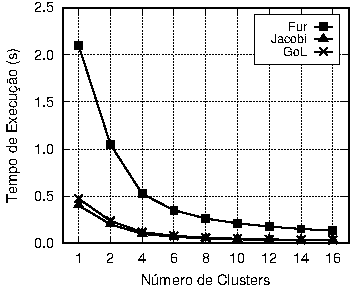
\includegraphics[width=0.4\textwidth]{figs/MPPAPlotScalabilityAPI.pdf}
% 	\legend{Fonte - o autor}
% 	\label{fig:escalabilidade}
% \end{figure}

% \begin{figure}[htb]
% 	\centering
% 	\caption{\textit{Tiles} vs. tempo (Fur).}
% 	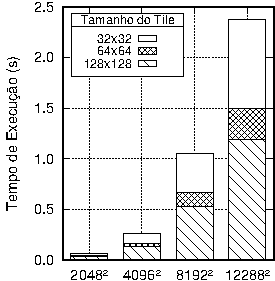
\includegraphics[width=0.4\textwidth]{figs/MPPAPlotAPIfurTimeTiles.pdf}
% 	\legend{Fonte - o autor}
% 	\label{fig:tiles}
% \end{figure}

% \begin{figure}[htb]
% 	\centering
% 	\caption{Tempo.}
% 	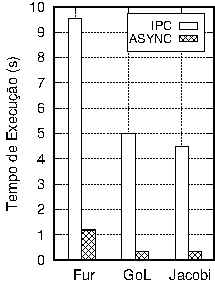
\includegraphics[width=0.4\textwidth]{figs/ComparisonTimeTiles1.pdf}
% 	\legend{Fonte - o autor}
% 	\label{fig:compara-tempo}
% \end{figure}

% \begin{figure}[htb]
% 	\centering
% 	\caption{Energia.}
% 	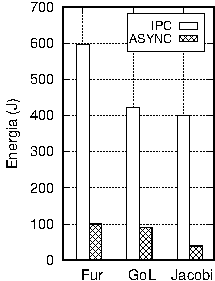
\includegraphics[width=0.4\textwidth]{figs/ComparisonEnergyTiles1.pdf}
% 	\legend{Fonte - o autor}
% 	\label{fig:compara-energia}
% \end{figure}